\documentclass{standalone}
\usepackage{tikz}
\begin{document}

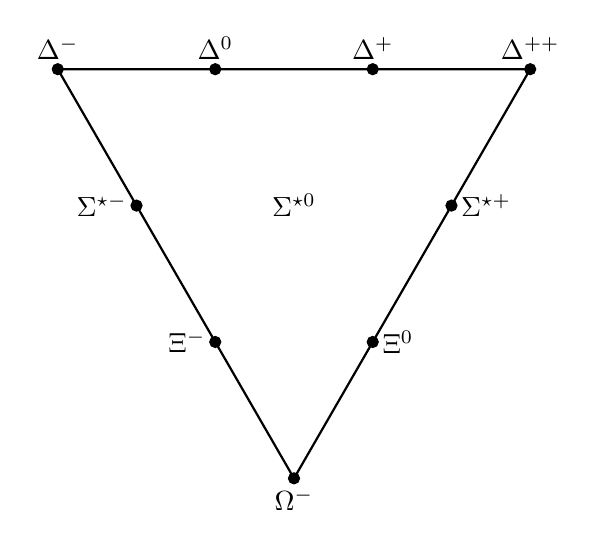
\begin{tikzpicture}

% Definir el tamaño del lado del triángulo equilátero
\def\side{6}

% Coordenadas de los vértices del triángulo equilátero (Delta-, Delta++, Omega-)
\coordinate (DeltaM) at (-\side/2, {sqrt(3)/2 * \side});
\coordinate (DeltaPP) at (\side/2, {sqrt(3)/2 * \side});
\coordinate (OmegaM) at (0, 0);

% Coordenadas de los puntos intermedios (Delta0, Delta+, Sigma*, Xi*)
\coordinate (Delta0) at (-\side/6, {sqrt(3)/2 * \side});
\coordinate (DeltaP) at (\side/6, {sqrt(3)/2 * \side});

\coordinate (SigmaM) at (-\side/3, {sqrt(3)/3 * \side});
\coordinate (Sigma0) at (0, {sqrt(3)/3 * \side});
\coordinate (SigmaP) at (\side/3, {sqrt(3)/3 * \side});

\coordinate (XiM) at (-\side/6, {sqrt(3)/6 * \side});
\coordinate (Xi0) at (\side/6, {sqrt(3)/6 * \side});

% Dibujar el triángulo equilátero
\draw[thick] (DeltaM) -- (OmegaM) -- (DeltaPP) -- cycle;

% Colocar etiquetas para cada partícula
\node[above] at (DeltaM) {$\Delta^-$};
\draw[fill=black] (DeltaM) circle (2pt);

\node[above] at (Delta0) {$\Delta^0$};
\draw[fill=black] (Delta0) circle (2pt);

\node[above] at (DeltaP) {$\Delta^+$};
\draw[fill=black] (DeltaP) circle (2pt);

\node[above] at (DeltaPP) {$\Delta^{++}$};
\draw[fill=black] (DeltaPP) circle (2pt);

\node[left] at (SigmaM) {$\Sigma^{\star -}$};
\draw[fill=black] (SigmaM) circle (2pt);

\node at (Sigma0) {$\Sigma^{\star 0}$};


\node[right] at (SigmaP) {$\Sigma^{\star +}$};
\draw[fill=black] (SigmaP) circle (2pt);

\node[left] at (XiM) {$\Xi^{-}$};
\draw[fill=black] (XiM) circle (2pt);

\node[right] at (Xi0) {$\Xi^{0}$};
\draw[fill=black] (Xi0) circle (2pt);

\node[below] at (OmegaM) {$\Omega^-$};
\draw[fill=black] (OmegaM) circle (2pt);

\end{tikzpicture}

\end{document}
